%/* vim: set filetype=latex */

% Demo project. Uses Komascript >=3.0. 
% which is not included in texlive 2008
% (1) copy dist to texlive/texmf-local 
% (2) texhash
%\documentclass[BCOR=8.5mm,DIV=calc,open=right,pagesize=auto,a5paper]{scrbook}
%\documentclass[12pt,BCOR=8.5mm]{scrbook}
%\documentclass[12pt,BCOR=8.5mm]{scrartcl}
\documentclass[logo]{fhgart}
\title{Power to the People}
\subtitle{Das Stromnetz der Zukunft}
\author{Mathias Dalheimer \texttt{<dalheimer@itwm.fhg.de>}}
%% PDF SETUP
\usepackage[pdftex, bookmarks, colorlinks, breaklinks,
pdftitle=\title,pdfauthor={Mathias Dalheimer},plainpages=false]{hyperref}  
\hypersetup{linkcolor=blue,citecolor=blue,filecolor=black,urlcolor=blue,plainpages=false} 

\clubpenalty=3000 % adjust for widows and orphans 10000 is max
\widowpenalty=3000 % adjust for widows and orphans 10000 is max
%% Font Adjustments
%\usepackage[LY1]{fontenc}
%\usepackage[T1]{fontenc}
%\usepackage{adobegaramond}
%\usepackage{gillsans}
%\renewcommand{\rmdefault}{HoeflerText}

% Use URW Garamond No. 8 as a default font. (getnonfreefonts)
%\usepackage[urw-garamond]{mathdesign}
%\renewcommand{\rmdefault}{ugm}
% Optima as a sans serif font.
%\renewcommand*\sfdefault{uop}

\newcommand*\imgwidth{0.8\textwidth}

\usepackage{ifthen}
\newboolean{InternalVersion}
\setboolean{InternalVersion}{true}
%\setboolean{InternalVersion}{false}

\usepackage{listings}  
\lstset{numbers=left, numberstyle=\tiny,numbersep=5pt}  
\lstset{language=Xml, basicstyle=\small, frame=shadowbox}  

\usepackage{algorithmic}
\usepackage{algorithm}
%\numberwithin{algorithm}{chapter} 
%\newcommand{\theHalgorithm}{\arabic{algorithm}}

\usepackage[protrusion=true,expansion=true]{microtype}

%% Page Header
\usepackage{scrpage2}

% Recalculate page setup based on new font.
%\KOMAoptions{DIV=last}
%\KOMAoptions{draft=true}

% Versals. 
%\usepackage{lettrine}
% Misc packages
\usepackage{url}
\usepackage{graphicx}
\usepackage{todonotes}
%\usepackage[english]{babel}
\usepackage{ngerman}
% Use utf-8 encoding for foreign characters
\usepackage[utf8]{inputenc}
\usepackage{blindtext}
\usepackage{subfigure}

\hyphenation{scho-oner Sur-vivor ap-pen-dix
Strom-ver-brauchs-informationen}

\usepackage{marvosym} % bei der Schrift enthalten
\newcommand*\euro{\textup{\EUR}}


%% Chapterstyle
%\renewcommand*{\chapterformat}{---\hskip.5cm\thechapter\hskip.5cm---}
%\KOMAoption{headings}{small,twolinechapter}
%\setkomafont{chapter}{\Large\sffamily\centering}
%\setkomafont{dictum}{\normalfont}
%\renewcommand*{\dictumwidth}{.8\textwidth}

%% Main.
\begin{document}
\maketitle
%\clearscrheadfoot
%\automark[chapter]{section}
%\lehead[]{\pagemark\hskip.5cm\vrule\hskip.5cm\title}
%\rohead[]{\headmark\hskip.5cm\vrule\hskip.5cm\pagemark} 
\title
%\pagestyle{scrplain}
%\begin{titlepage}
%%/* vim: set filetype=tex */

%\vspace*{\baselineskip} 
\vfill 
\hbox{% 
\hspace*{0.2\textwidth}% 
\rule{1pt}{\textheight} 
\hspace*{0.05\textwidth}% 
\parbox[b]{0.75\textwidth}{ 
\vbox{% 
%\vspace{0.1\textheight} 
{\noindent\huge\sffamily \title\\[0.5\baselineskip] }
\\[2\baselineskip] 
{\Large\sffamily \subtitle}\\[4\baselineskip] 
{\Large\sffamily \author }
\\[\baselineskip] 
{\Large\sffamily dalheimer@itwm.fhg.de}\par
\vspace{0.5\textheight} 
{\noindent Auf dem Weg zum Energiesystem für die nächsten 50 Jahre}\\[\baselineskip] 
}% end of vbox 
}% end of parbox 
}% end of hbox 
\vfill 
%\null 

%\end{titlepage}
%% frontmatter
%%\input{frontmatter}
%%\parindent.0cm
%%\parskip.4cm
%%\input{pagetwo}
%\parindent.4cm
%\parskip.0cm
%\pagestyle{scrheadings}
%
\section{Einleitung}


Wenn morgens in Deutschland die Kaffeemaschinen angeschaltet werden,
sorgt ein komplexes System dafür, dass der Tag gut anfängt: Unser
Stromnetz. Das deutsche Stromnetz ist über die vergangenen 100 Jahre
gewachsen und transportiert den Strom von Kraftwerken zu den
Verbrauchern. Bildlich kann man sich das anhand des "`Stromsees"' vor
Augen führen:

\begin{figure}[htbp]
  \begin{center}
    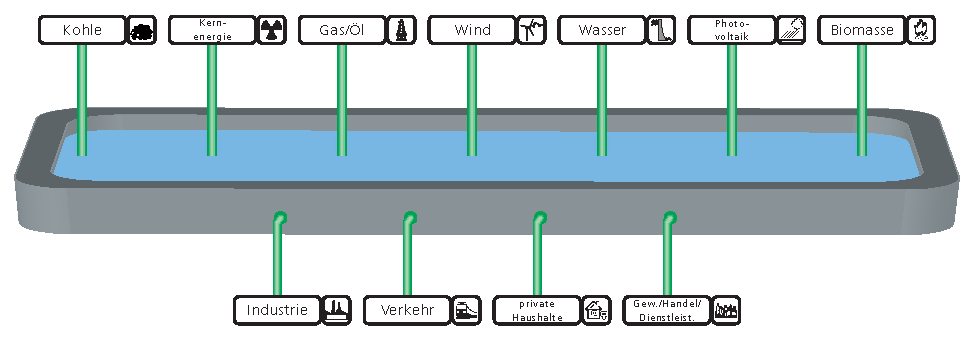
\includegraphics[width=\imgwidth]{figures/stromsee}
    \caption{Der Stromsee: Kraftwerke erzeugen Strom, der in den
    gemeinsamen Stromsee engespeisst wird. Alle Verbraucher beziehen 
    ihren Strom aus diesem Netz.}
    \label{fig:figures/stromsee}
  \end{center}
\end{figure}


Die einzelnen Kraftwerke produzieren aus verschiedenen Energiequellen
elektrischen Strom. Der Strom wird im Netz gesammelt, bis ein beliebiger
Verbraucher den Strom benötigt\footnote{Streng genommen wird Strom
natürlich nicht verbraucht, ich bleibe allerdings bei dieser
umgangssprachlichen Formulierung.}. Konventionelle Kohlekraftwerke
tragen genauso wie Atomkraftwerke und Photovoltaiksysteme zur
Stromerzeugung bei. Das Stromnetz wird mit einem Wasserleitungssystem
verglichen.  So anschaulich dieses Modell ist, so vereinfacht es
leider zu stark:

\begin{enumerate}
  \item Der Stromsee suggeriert, dass der "`Wasserstand"' im See steigen
    und fallen kann. Das ist im Stromnetz nicht möglich, es gibt keinen
    Speicher, der Abweichungen zwischen Erzeugung und Verbrauch
    kompensieren könnte:
    \begin{equation}
      \textrm{Erzeugung}(t) = \textrm{Verbrauch}(t) + \epsilon \hspace{1cm} \forall t
    \end{equation}
    Die Erzeugung muss zu jedem Zeitpunkt dem Verbrauch entsprechen ---
    kleinere Abweichungen führen zur Änderung der Netzfrequenz, größere
    Abweichungen können zu großflächigen Stromausfällen führen. Es ist
    die Aufgabe der Stromnetzbetreiber, einen zuverlässigen Betrieb
    sicherzustellen. Dazu wird die Stromerzeugung permanent dem
    Verbrauch angepasst~\cite[S. 33ff]{schwab06elektroenergiesysteme}. Es ist
    nicht möglich, beliebige Kapazitäten bei Bedarf an- und
    abzuschalten: Die Anfahrvorgänge von Kraftwerken dauern je nach
    Kraftwerkstyp zwischen wenigen Minuten (Wasserkraft- und
    Gasturbinenkraftwerke) und mehreren Stunden (Kohlekraftwerke).
    Umgekehrt ist es auch nicht ohne weiteres möglich, die Leistung
    innerhalb von kurzer Zeit beliebig zu reduzieren. 

    \begin{figure}[htbp]
      \begin{center}
        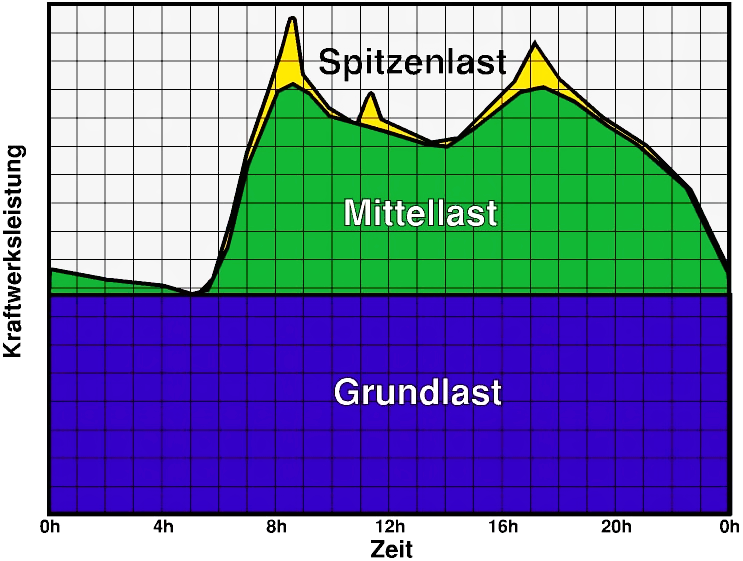
\includegraphics[width=\imgwidth]{figures/Stromnetz_Lastkurve.png}
        \caption{Lastkurve. Quelle: \url{http://de.wikipedia.org/w/index.php?title=Datei:Stromnetz_Lastkurve.png}}
        \label{fig:stromnetz_lastkurve}
      \end{center}
    \end{figure}
    
    Die Netzbetreiber müssen also die Schwankungen des Stromverbrauchs
    vorhersagen und auch kurzfristig auf Änderungen reagieren. Dabei
    unterscheidet man zwischen Grund-, Mittel- und Spitzenlast, vlg.
    Abbildung~\ref{fig:stromnetz_lastkurve}: Die
    Grundlast ist der Bedarf, der über 24 Stunden hinweg konstant
    bleibt, quasi der Grundverbrauch. Dieser wird üblicherweise durch
    Grundlastkraftwerke wie Braunkohle- und Atomkraftwerke erzeugt. Auch
    Laufwasserkraftwerke werden üblicherweise zu den
    Grundlastkraftwerken gerechnet. Die Regelfähigkeit dieser Kraftwerke
    spielt eine untergeordnete Rolle, die Stückkosten stehen im
    Vordergrund: Die Erzeugung einer Kilowattstunde ist in diesen
    Kraftwerken am billigsten. Daher werden diese Kraftwerke wenn
    möglich rund um die Uhr unter Volllast betrieben.

    Die Mittellast entspricht den grundlegenden Schwankungen im
    Tagesablauf: Nachts wird erheblich weniger Energie verbraucht als
    tagsüber. Die Mittellast ist relativ gut planbar und
    wird daher z.B. mittels Steinkohlekraftwerken abgedeckt. Die
    Spitzenlast ist zwar auch planbar, aber mit erheblich mehr
    Unsicherheit verbunden. Diese Spitzenlast muss kurzfristig durch das
    Zuschalten von Spitzenlastkraftwerken wie Gasturbinenkraftwerken,
    Pumpspeicherkraftwerken oder Druckluftspeicherkraftwerke abgedeckt
    werden. Spitzenlastkraftwerke können ihre Leistung zum Teil bis zu
    20\% ihrer Nennleistung innerhalb einer Minute
    ändern~\cite{wikipedia10spitzenlast}\cite[S.
    108ff]{schwab06elektroenergiesysteme}. Da Spitzenlastkraftwerke nur
    selten unter Volllast betrieben werden, ist der erzeugte Strom
    relativ teuer: Je nach Versorgungslage kann eine Kilowattstunde
    \euro $1,50$ kosten~\cite{wikipedia10regelleistung}\cite[S.
    60]{schwab06elektroenergiesysteme}. 

    Nicht in die aktive Netzregelung einbezogen sind Industriebetriebe
    mit eigener Stromerzeugung, Windkraftanlagen, Photovoltaiksysteme
    und auch Blockheizkraftwerke. 

    Für die Regelung hat das "`European Network of Transmission System
    Operators for Electricity"' (ENTSO-E) Standards geschaffen. Im
    "`UCTE Operation Handbook"' sind die Verfahren der Netzregelung im
    Abschnitt "`Load Frequency Control and Performance"'
    beschrieben~\cite{entsoe10ucte}. Als Regelgröße dient die
    Netzfrequenz: Dieser Wert muss bei 50 Hz liegen. Wenn ein
    elektrischer Verbraucher eingeschaltet wird, dann sinkt die
    Netzfrequenz. Wird umgekehrt ein Verbraucher ausgeschaltet, so
    steigt die Netzfrequenz. Genau umgekehrt wird die Netzfrequenz von
    der Leistung der Kraftwerke beeinflusst: Wird zusätzliche Leistung
    eingespeisst, so steigt die Netzfrequenz.

    Drei aufeinanderfolgende Stufen sind an der Regelung beteiligt:
    \begin{enumerate}
      \item Für die \emph{Primärregelung} müssen Netzbetreiber innerhalb
        von 30 Sekunden zwei Prozent seiner aktuellen Erzeugung als
        Reserve bereitstellen bzw. die Erzeugung reduzieren können. Die
        Kraftwerke müssen bis zu 15 Minuten diese Leistungserhöhung
        liefern können. Die Primärregelung hat die Aufgabe, die
        Netzfrequenz im Höchstspannungsnetz auf europäischer Ebene
        stabil zu halten.
      \item Die \emph{Sekundärregelung} kann zeitgleich zur
        Primärregelung anlaufen und hat die Aufgabe, die
        Frequenzstabilität in einer Regelzone sicherzustellen. Dazu
        werden zusätzliche Spitzenlastkraftwerke benutzt. Die
        Sekundärregelung soll nach 15 Minuten abgeschlossen sein.
      \item Auch bei der \emph{Tertiärregelung} oder auch
        \emph{Minutenreserve} ist das Ziel, die Netzfrequenz zu
        stabilisieren. Hierbei werden zusätzliche Reserven vom
        Übertragungsnetzbetreiber bei den Lieferanten angefordert. Dies
        geschieht üblicherweise telefonisch. Die veränderte
        Lastsituation wird dann permanent durch die Kraftwerke
        abgedeckt, die Regelung ist abgeschlossen.
    \end{enumerate}

  \item Der Stromsee vernachlässigt auch, dass die Erzeugung und der
    Verbrauch von Strom geographisch verteilt sind. Eine Kilowattstunde
    aus einem Grundlastkraftwerk wird normalerweise in das
    Höchstspannungsnetz (220 und 380 Kilovolt) eingespeist, vgl. Tabelle
    \ref{tab:stromkreise}. Die Aufgabe des Höchstspannungsnetzes ist die
    Verteilung des Stroms über größere Distanzen, auch in das
    europäische Ausland. Nahe den Verbrauchszentren wird der Strom in
    das Hochspannungsnetz transformiert, von dort aus auch in das
    Mittelspannungsnetz. Mittelgroße Kraftwerke speisen in das
    Hochspannungsnetz ein, während Stadtwerke und große Windkraft- bzw.
    Photovoltaikanlagen auch direkt in das Mittelspannungsnetz
    einspeisen können. 

    \begin{table}
    \centering
    \begin{tabular}{|l|r|r|}
      \hline
      & Installierte Länge (km) & Spannung (kV) \\
      \hline
      Höchstspannung & 36.000 & 220 und 380 \\
      Hochspannung & 75.200 & 60-220 \\
      Mittelspannung & 493.000 & 6-60 \\
      Niederspannung & 1.067.100 & 0,4\\
      \hline
    \end{tabular}
    \caption{Stromkreise in Deutschland. Quelle: BMWi~\cite{bmwi10stromnetze}}
    \label{tab:stromkreise}
  \end{table}
 
    Über Umspannwerke in den Gemeinden wird das Mittelspannungsnetz an
    das Niederspannungsnetz angeschlossen. Hier wird der Strom
    schließlich durch private Haushalte und Gewerbebetriebe verbraucht.
    Eine Ausnahme stellen Industrieabnehmer dar: Diese können ihren
    Strom auch aus dem Mittelspannungsnetz beziehen.

    Die Einspeisung von Solaranlagen auf den Dächern der Privathaushalte
    kann zu Problemen bei der Netzregulierung führen: Da auf der
    Niederspannungsebene keine Regelenergie zur Verfügung steht, können
    signifikante Photovoltaikeinspeisungen die Netzfrequenz nach oben
    treiben. Darüber hinaus kann eine Einspeisung von dezentral
    erzeugtem Solarstrom auch die Leitungen als solche überlasten.
    Daher kommt es schon heute --- vor allem in ländlichen Regionen ---
    vor, dass die Netzbetreiber den Anschluss von Photovoltaikanlagen
    verweigern.
   
  \item Der Stromsee stellt schließlich auch die Organisationsstruktur
    des Stromnetzes nicht dar. Hier sind zunächst die vier großen
    Übertragungsnetzbetreiber Amprion (RWE/VEW), EnBW Transportnetze AG,
    Transpower Stromübertragungs GmbH (TenneT) sowie 50Hertz
    Transmission (Vattenfall) zu nennen, vgl. Abbildung
    \ref{fig:regelzonen}.  \begin{figure}[htbp] \begin{center}
      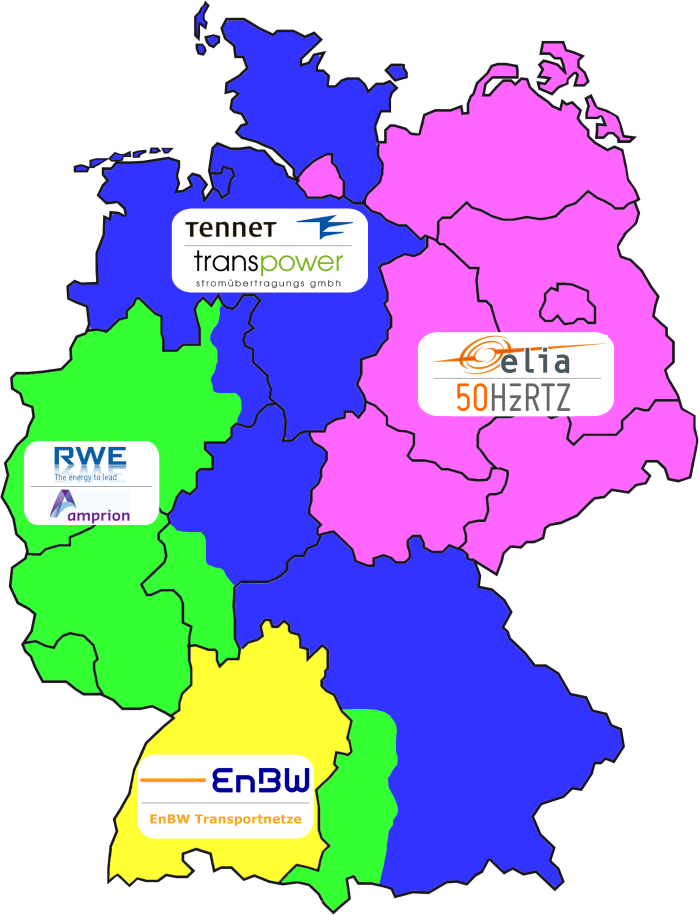
\includegraphics[width=\imgwidth]{figures/Regelzonen_deutscher_Netzbetreiber_neu.png}
      \caption{Überblick über die Regelzonen im deutschen Stromnetz.
      CC-BY-SA Ice gixxe} \label{fig:regelzonen} \end{center}
    \end{figure}
%http://de.wikipedia.org/w/index.php?title=Datei:Regelzonen_deutscher_%C3%9Cbertragungsnetzbetreiber_neu.png&filetimestamp=20100621164106
    Die vier großen Übertragungsnetzbetreiber sind am ENTSO-E beteiligt
    und damit auch an der aktiven Netzregelung. Sie betreiben die
    Höchst- und Hochspannungsnetze. Hinzu kommen noch ca. 900
    Verteilnetzbetreiber in Deutschland, welche die Mittel- und
    Niederspannungsnetze betreiben. Diese agieren lokal und stellen die
    Versorgung der Haushalte in ihrem Versorgungsgebiet sicher. Oft sind
    diese Verteilnetzbetreiber in der Hand der Kommunen.

    Alle Netzbetreiber kaufen --- direkt oder indirekt --- ihren Strom
    auf zwei Märkten ein: Der Termin- und der Spotmarkt an der European
    Energy Exchange (EEX) in Leipzig. Auf dem Terminmarkt werden
    längerfristige Lieferkontrakte gehandelt. Der Spotmarkt dient
    hingegen dem An- und Verkauf von Strommengen für den folgenden oder
    auch laufenden Tag. Hier können kurzfristig Strommengen ge- und
    verkauft werden für den Fall, dass die bisherigen Käufe nicht mit
    dem erwarteten Verbrauch übereinstimmen.

    Die Erzeugung des Stroms wird in Deutschland von den vier Konzernen
    Vattenfall, RWE, e-on und EnBW dominiert. Daneben gibt es eine
    große Anzahl von Stadtwerken, die mit eigenen Kraftwerken Strom
    erzeugen. Hinzu kommt noch eine Vielzahl von kleinen Erzeugern, die
    mittels BHKW und Photovoltaik lokal Strom in das Netz einspeisen.
    Die Monopolkommission der Bundesregierung stellte in ihrem Gutachten
    "`Strom und Gas 2009"' fest, dass insbesondere im Bereich der
    Stromerzeugung signifikante Wettbewerbsprobleme aufgrund der hohen
    Marktkonzentration vorliegen. Sie empfiehlt unter anderem eine
    Zusammenlegung der vier Regelzonen zu einer einzigen, unter einer
    unabhängigen Regelinstanz operierenden Regelzone
    \cite{monopolkommission09stromgas}. 
\end{enumerate}

Unser Stromnetz ist also weit komplexer als der Stromsee suggeriert.  Der
Ausbau der erneuerbaren Energien verändert dabei viele der
Grundannahmen, unter denen unser Stromnetz gebaut wurde. Da der
Netzbetreiber die Einspeisungen von Solaranlagen entgegennehmen und
vergüten muss, sind sowohl technische Änderungen als auch
organisatorische Anpassungen nötig.

Die Stromerzeugung aus Wind, Photovoltaik und Biomasse hat einen
steigenden Anteil, im Jahr 2009 betrug er
15,6~\%~\cite{web:bmwi-energiedaten}.  Die Tendenz ist weiter steigend,
einzelne Studien gehen von einem Anteil zwischen mindestens 20
~\%~\cite{dena05netzstudie1} und 47~\% ~\cite{iwes09simulation} der
Erneuerbaren Energien bis 2020 aus.  Grundsätzlich macht dieser Trend
aus ökologischer Sicht Sinn.  Die unregelmässige Verfügbarkeit des
EE-Stromes führt dazu, dass z.B. in Phasen starken Windes
Grundlastkraftwerke heruntergefahren werden müssen, um die zusätzlichen
Strommengen aufzunehmen. Die Machbarkeit ist hier umstritten:
Gegner der erneuerbaren Energien weisen darauf hin, dass
Grundlastkraftwerke nicht ohne weiteres innerhalb von Stunden
heruntergefahren werden können.  Befürworter halten dagegen, dass
aufgrund von speziellen Windprognosen die Stromeinspeisungen auf
Tagesfrist recht genau vorhergesagt werden können und daher eine
Abschaltung von Kohle- und Atomkraftwerken machbar ist.

Klar ist in jedem Fall, dass sich durch den zunehmenden Anteil
regenerativer Energien im deutschen Strommix Grundlastkraftwerke immer
schlechter auslasten lassen.  Es verändert sich auch die finanzielle
Grundlage für den Betrieb von Grundlastkraftwerken: Diese sind darauf
optimiert, möglichst permanent mit hoher Auslastung Strom zu
produzieren. 

Das derzeit praktizierte Anhalten von Windkraftanlagen in Phasen starken
Windes durch die Netzbetreiber ist aus ökologischer Sicht nicht
wünschenswert. Die Gründe hierfür liegen laut der Bundesregierung zum
einen an Verzögerungen im Netzausbau und andererseits im Fehlen von
Energiespeichern~\cite{bundesreg2010kleineanfrage}. Der Anteil des nicht
eingespeisten regenerativen Stroms wird derzeit nicht erfasst. Dies ist
bedauerlich, da die Netzbetreiber auch Betreiber von
Grundlastkraftwerken sind und so ein Zielkonflikt entsteht.

Zusammenfassend lässt sich festhalten: Erneuerbare Energien --- so
wünschenswert ihr Einsatz ist --- führen zu Veränderungen im Stromnetz.
Neben technischen Anpassungen sind auch ökonomische Anpassungen
notwendig. Wohin also mit dem "`grünen"' Strom? Wie kann unser Stromnetz
angepasst werden?

\section{Flexibel durch Demand-Side Management}\label{sec:demand-side_management}

Klar ist, dass unser Stromnetz flexibler werden
muss~\cite{geller2010smartgrid}. Prinzipiell gibt es zwei Möglichkeiten,
dies zu schaffen: Einerseits können Speichermöglichkeiten für Strom im
Netz geschaffen werden, andererseits kann die Nachfrage nach Strom an
das Angebot angepasst werden. In Pumpspeicherkraftwerken kann Strom
zwischengespeichert werden, in dem Wasser von einem niedrigen Reservoir
in ein höher gelegenes gepumpt wird.  Wird der Strom wieder benötigt, so
wird die in der Höhe gespeicherte Energie über ein Wasserkraftwerk
wieder in Strom verwandelt.  Üblicherweise werden Pumpspeicherkraftwerke
so dimensioniert, dass sie über 4-8 Stunden ihre Leistung abgeben
können. Dabei steht die Leistung innerhalb von Minuten zur Verfügung und
kann in weiten Bereichen geregelt werden. Der Wirkungsgrad liegt bei ca.
75~\%~\cite[S. 175]{schwab06elektroenergiesysteme}.

Strom kann auch in Druckluftspeichern zwischengespeichert werden. Diese
Technik ist jedoch nicht weit verbreitet --- weltweit existieren nur
zwei Kraftwerke dieser Bauart, eines davon im niedersächsischen
Huntorf~\cite{web11huntorf}. Druckluftspeicher benötigen geologisch geeignete,
luftdichte Salzstöcke und können daher nicht überall errichtet werden.
Entlang der Nordseeküste könnten allerdings in Zukunft entsprechende
Standorte genutzt werden, um Erzeugungsspitzen von Windanlagen
aufzunehmen und später wieder an das Netz abzugeben. 

In Schwungrädern kann ebenso Strom zwischengespeichert werden. Die
Energiedichte ist hier sehr hoch, allerdings kann in Schwungrädern nur
relativ wenig Energie gespeichert werden. Schwungräder werden daher
überwiegend zur Netzstabilisierung eingesetzt.

Eine weitere Möglichkeit zur Stromspeicherung liegt in modernen
Batteriespeichern. Hier gibt es verschiedene Technologien: Neben
Lithium-Ionen-Batterien werden auch Redox-Flow-Zellen oder
Natrium-Schwefel-Hochtemperaturzellen in Betracht gezogen. Allen
Speichern ist gemeinsam, dass Strom in chemische Energie umgewandelt
wird. Je nach Batterietyp erfordert die Ladung des Speichers eine
komplexe Laderegelung und spezielle Sicherheitsvorkehrungen. Die
Lebensdauer von Batterien wird erheblich durch die Betriebsparameter
beeinflusst.

Es gibt derzeit erste Projekte, die den
großtechnischen Einsatz von Lithion-Ionen-Batterien
erproben~\cite{braun09lithium}. Dabei werden dezentral Batteriespeicher
installiert, die im Falle eines Überschusses Strom aufnehmen und später
wieder abgeben können. In die gleiche Kategorie fallen auch
Elektrofahrzeuge, die ihre Batteriekapazität nach aussen hin zugänglich
machen. Technisch sind stationäre Systeme jedoch einfacher zu betreiben:
Die Lade- und Entladeregelung muss nicht die hohen Leistungen zur
Verfügung stellen, die in einem Elektroauto notwendig sind. Darüber
hinaus werden stationäre Systeme auch nur bis zu 30~\% ihrer Kapazität
entladen. Mit aktuell verfügbaren Technologien können so
Batterielebenszeiten von 25 Jahren erreicht werden. Dezentrale
Batteriespeicher haben auch den Vorteil, dass sie direkt am
Niederspannungsnetz hängen und so z.B. die Einspeisungen von privaten
Photovoltaiksystemen aufnehmen können. Der so zwischengespeicherte Strom
belastet die Übertragungsnetze nicht, sondern verbleibt lokal in einem
Versorgungsnetz, bis der Strom dort benötigt wird.

Die zweite Möglichkeit, das Stromnetz flexibler zu machen, liegt im \emph{Demand-Side
Management}. Statt auf der Seite der Stromerzeugung und -verteilung
Änderungen vorzunehmen, wird der Verbrauch von Strom beeinflusst. Damit
ist jedoch zunächst nicht die Reduzierung des Stromverbrauchs gemeint,
obwohl dies natürlich eine sinnvolle Anstrengung ist. Stattdessen wird
der Stromverbrauch auf der Zeitachse verschoben. Das Ziel ist es,
Stromverbraucher dann zu betreiben, wenn sowieso viel Strom erzeugt
wird. Umgekehrt laufen diese Verbraucher nicht, wenn zu einem anderen
Zeitpunkt weniger Strom erzeugt wird.

Im Industriebereich ist diese Herangehensweise schon lange Standard ---
unter dem Stichwort "`Lastabwurf"' hat ein Netzbetreiber die
Möglichkeit, den Stromverbrauch von einzelnen Industriebetrieben gezielt
zu reduzieren, um Engpässe zu vermeiden. Im Gegenzug erhält der
Industriebetrieb bessere Bezugskonditionen für Strom. Ein
Verteilnetzbetreiber ist so in der Lage, relativ schnell erhebliche
Lasten im Netz der momentanen Erzeugung anzupassen. Üblicherweise sind
--- unter anderen --- die folgenden Eingriffe möglich \cite[S.
23f]{wiechmann08lastmanagement}~\cite[S. 85ff]{bmwi06eenergy}:

\begin{enumerate}
  \item \emph{Lastspitzenreduzierung:} Dabei werden einzelne Lastspitzen
    gekappt, in dem zur Spitzenzeit Verbraucher abgeschaltet werden. In
    den Spitzenzeiten werden so höhere Kosten zur Stromerzeugung
    vermieden.
  \item \emph{Lasttalauffüllung:} Falls Strom zu Grenzkosten angeboten
    werden kann, lohnt es sich, Verbraucher zu diesem Zeitpunkt zu
    betreiben. Ein Tiefkühlhaus könnte in solchen Phasen als
    Energiespeicher dienen, in dem die Temperatur abgesenkt wird. Durch
    diese Temperaturabsenkung wird dann später weniger Strom benötigt.
    Gleichzeitig werden eventuelle Überschüsse sinnvoll genutzt.
  \item \emph{Lastverschiebung:} Generell können natürlich Lasten im
    Stromnetz auf einen anderen Zeitpunkt verschoben werden, um
    vielfältige Ziele zu erreichen. Speziell bei kurzfristigen
    Lastveränderungen ("`Flexible Load Shaping"') wird kurzfristig
    Regelenergie durch einen Lastabwurf frei.
\end{enumerate}

Allen Eingriffen gemein ist, Lastspitzen zu glätten oder zu verschieben,
um den Einsatz teurer Spitzenlastkraftwerke zu verhindern. Bei
entsprechenden Prognosen können diese Techniken auch dazu eingesetzt
werden, Strom aus den erneuerbaren Energiequellen aufzunehmen und
gezielt zu nutzen. Im Jahr 2007 nutzen die europäischen
Übertragungsnetzbetreiber Demand Side Management-Kapazitäten im Bereich von
mehreren GWh~\cite{etso07demand}. Torriti et al.~\cite{torriti10demand}
gehen von einem stetigen Wachstum der Kapazitäten in Europa aus, vgl.
Tabelle \ref{tab:drforecast}. Zusammengenommen können momentan 2,9~\% der
Spitzenlast durch Demand Side Management verschoben werden.

\begin{table}
  \centering
  \begin{tabular}{|l|r|}
    \hline
    Jahr & Kapazität in GW \\
    \hline
    2008 & 11,45\\
    2010 & 11,50\\
    2013 & 12,15 \\
    2015 & 12,82 \\
    2020 & 13,32 \\
    \hline
  \end{tabular}
  \caption{Prognose der Demand Side Management-Kapazitäten im Bereich
  der UCTE. Quelle: \cite{torriti10demand}}
  \label{tab:drforecast}
\end{table}

Im Privathaushalt ist Demand Side Management jedoch noch nicht im
Einsatz, hier können noch erhebliche Kapazitäten erschlossen werden. Die
Gründe hierfür sind vielfältig: 

\begin{enumerate}
  \item Die notwendige Regelungstechnik ist in nur wenigen Haushalten
    vorhanden. Die Grundlage für die Steuerung von Geräten ist ein
    Hausbus, über den Steuersignale kommuniziert werden. Die gegenwärtig
    verfügbaren Systeme (KNX, EIB) sind recht aufwendig und teuer,
    sodass hier noch weitere Entwicklungen notwendig sind.
  \item In die Haushaltsgeräte ist normalerweise kein Zugang für ein
    Energiemanagementsystem eingebaut. Zum Beispiel gibt es bei einer
    Spülmaschine üblicherweise keine Schnittstelle, um ein Startkommando
    zu übermitteln.
  \item Es gibt kaum finanzielle Anreize für Privathaushalte, um in
    diese Technologien zu investieren. Gegenwärtig sind einzig
    Nachtstromtarife darauf zugeschnitten, den Verbrauch in Nebenzeiten
    zu fördern. Diese Tarife fördern jedoch eher den Betrieb von
    Grundlastkraftwerken als den sinnvollen Verbrauch von Strom zu
    Zeiten hoher Ökostromproduktion.
\end{enumerate}


Im Rahmen der E-Energy Initiative der Bundesregierung arbeiten diverse
Projekte daran, Demand Side Management-Technologien in Haushalte zu
integrieren~\cite{web:e-energy}. Auch Gerätehersteller wie Miele
integrieren spezielle Energiemanagementschnittstellen in ihre
Geräte~\cite{miele10ifapresse}. Allen diesen Lösungen gemein ist jedoch,
dass sie modellhaften Charakter haben und allenfalls in Pilotprojekten
getestet werden.

In diesen Pilotprojekten ist neben den Managementtechnologien vor allem
die Einführung von intelligenten Stromzählern (Smart Metern) ein Thema.
Smart Meter sind elektronische Stromzähler, welche die bekannten
schwarzen Ferraris-Zähler ersetzen. Sie bieten neben der Anzeige des
Gesamtzählerstandes auch die Möglichkeit, den Momentanverbrauch oder den
Wochenverbrauch anzuzeigen. Einige Modelle bieten zudem auch die
Möglichkeit, den Stromverbrauch an den Netzbetreiber zurückzumelden, oft
in 15-minütigen Intervallen. Stromkunden können, wenn
Informationen zum Momentanverbrauch unmittelbar zur Verfügung stehen,
ihr Verhalten direkt verändern und so ihren Strombezug um 15-20~\%
reduzieren~\cite{geller2010smartgrid}. Ebenso ist es denkbar, mit den
gesammelten Strombezugsinformationen weiterführende Analysen
durchzuführen. Diese können zum Beispiel Geräte identifizieren, die
einen erheblichen Anteil am Stromverbrauch haben. Daraufhin können
automatisiert Hinweise gegeben werden, dass sich z.B. die Anschaffung
eines energiesparenden Kühlschranks schon nach einem Jahr amortisiert
hätte.

Für die Netzbetreiber bzw. den Messtellenbetreiber ist dies eine
Herausforderung, da Kunden nicht bereit sind, für die neue Messtechnik
zu bezahlen. Zwar sind durch die direkte Rückmeldung von
Stromverbrauchsdaten Einsparungen zu erwarten,
jedoch stehen diese Einsparpotentiale in keinem Verhältnis zu
den Mehrkosten der Smart Meter: Die Bundesnetzagentur geht von einem
Einsparpotential von 12\euro bis 50\euro im Jahr
aus~\cite[S. 70]{bundesnetzagentur10handlungsoptionen}. Zudem erlauben gerade zeitlich eng
aufgelöste Daten im 15-Minuten-Bereich erhebliche Rückschlüsse auf die
Lebensgewohnheiten der Anschlussinhaber.


\section{Datenschutz}\label{sub:datenschutz}
Einerseits sind diese Daten natürlich für den Stromkunden interessant,
da er den Einfluss seines Verhaltens auf den Stromverbrauch vor Augen
geführt bekommt und so insgesamt weniger verbrauchen wird.  
Andererseits sind die Stromverbrauchsdaten aus Netzbetreibersicht auch
sehr interessant, da sich hier völlig neue Möglichkeiten für
Preismodelle und auch für das Marketing ergeben. Momentan werden
Privathaushalte über Standardlastprofile abgerechnet, d.h. ein
Verteilnetzbetreiber wird nicht für die real gelieferte Strommenge
bezahlt, sondern auf der Basis eines durchschnittlichen Lastprofils und
der Anzahl der versorgten Haushalte wird eine Pauschale abgerechnet. Mit
Smart Metern kann nun der reale Verbrauch bestimmt werden und wird in
Zukunft wohl zur Grundlage der Abrechnung werden \footnote{Entsprechende
Änderungen werden derzeit von der Bundesnetzagentur diskutiert.}. 

Um diese Abrechnung vorzunehmen gehen die Netzbetreiber davon aus, dass
die Stromverbrauchsdaten in hoher zeitlicher Auflösung an sie übertragen
werden, um dann eine verbrauchsgenaue Abrechnung gegenüber den
Stromanbietern machen zu können. Diese Daten sind jedoch als sehr
sensibel einzustufen, da hieraus auf Lebens- und Konsumgewohnheiten
geschlossen werden kann. 

Ein beispielhafter Tagesverlauf des Autors ist in Abbildung
\ref{fig:schlaflos} dargestellt.
\begin{figure}[htbp]
  \begin{center}
    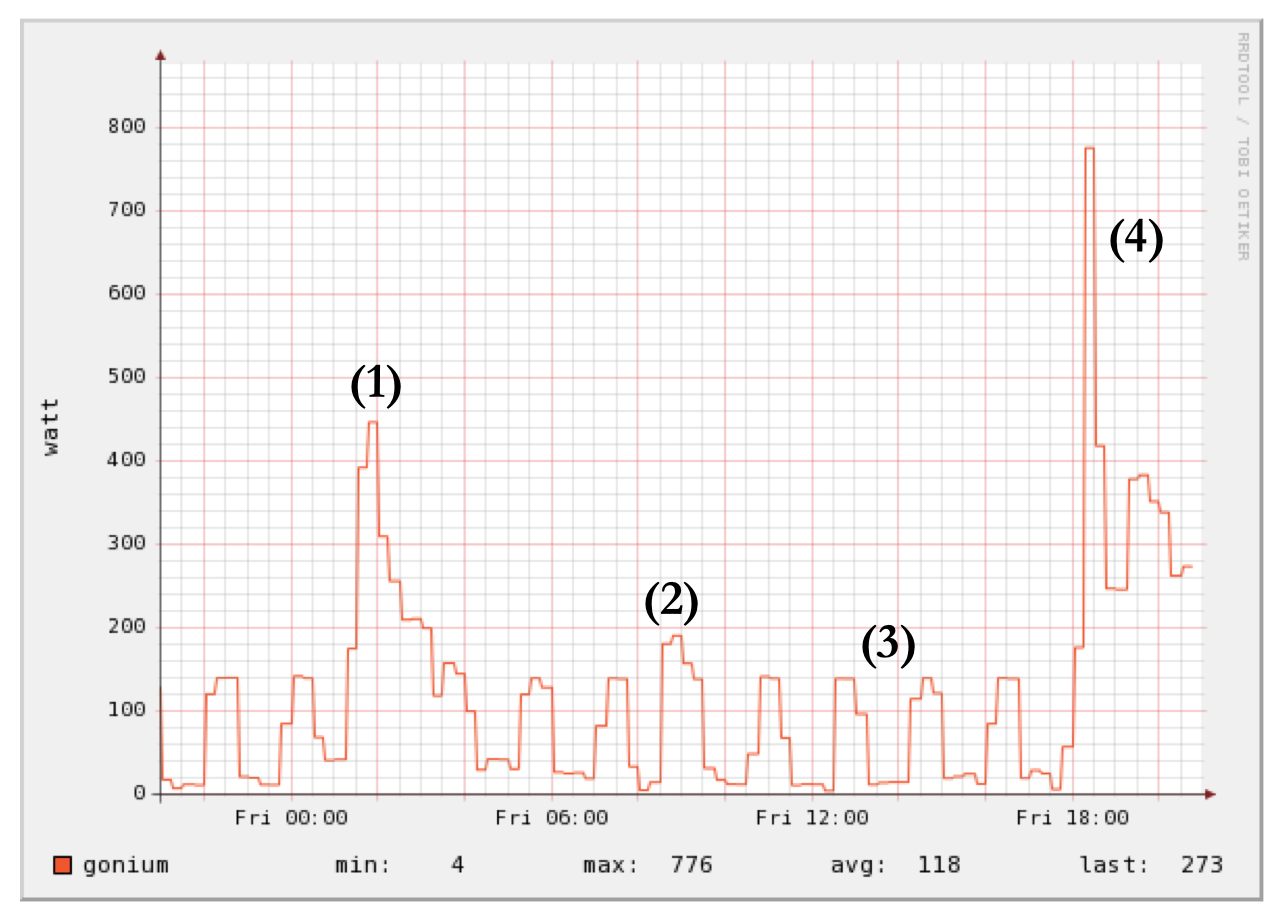
\includegraphics[width=\imgwidth]{figures/lastkurve-md-annotated.png}
    \caption{Der Stromverbrauch des Autors am Beispiel eines Tages.}
    \label{fig:schlaflos}
  \end{center}
\end{figure}
Die Kurve gibt den Stromverbrauch in fünfminütigen Intervallen
wieder. Bei Markierung (1) ist der Autor aufgestanden, weil er aufgrund
einer Kanada-Reise an Jetlag litt. Die Benutzung von Wasserkocher und
der Rechners schlägt sich deutlich nieder. Gegen 4:00 wurde
weitergeschlafen. Um acht Uhr morgens (2) läuft die kleine
Senseo-Kaffeemaschine, tagsüber war der Autor arbeiten. Während dieser
Zeit führt der Kühlschrank zu regelmässigen Ausschlägen (3). Gegen 18:00
kam der Autor nach Hause und benutzte die Mikrowelle.

Die Gerätesignaturen sind natürlich spezifisch für einzelne Geräte bzw.
Betriebszustände. Eine Waschmaschine bietet verschiedene Programme, die
auch zu leicht unterschiedlichen Signaturen führen. Zusätzlich führt die
Reduktion auf --- in diesem Beispiel --- fünf-Minuten-Messintervalle zum
Verlust von Information. Die Senseo-Kaffeemaschine (2) zeigt bei
einminütigen Messintervallen einen recht spezifischen Spitzenverbrauch
von 1400 Watt für ca. 1 Minute. Wenn die Werte jedoch als
Durchschnittsverbrauch der letzten fünf Minuten dargestellt werden,
bleibt davon nur noch eine kleine Spitze übrig.

Derzeit sehen die Smart Meter-Infrastrukturen eine zeitnahe Übermittlung
von 15-Minuten-Intervallwerten an die Messstellenbetreiber vor. Daraus
lassen sich immer noch einzelne Geräte identifizieren, wobei natürlich
wenig charakteristische Signaturen herausgemittelt
werden\footnote{Auch hier gilt natürlich das Nyquist-Theorem.}. Dennoch
ergeben sich hier erhebliche Privacy-Probleme: Durch statistische
Verfahren lässt sich recht einfach entscheiden, wie oft und wie lange
ein Bewohner in der Wohnung ist. Daraus kann zum Beispiel abgeleitet
werden, ob der Bewohner einer regelmässigen Tätigkeit
nachgeht~\cite{mueller10verhalten}~\cite{kurz10smartmeter}. 

Derzeit argumentieren die Messstellenbetreiber, dass die Installation
von Zählern und die Übertragung und Speicherung von Verbrauchsdaten für
die Abrechnung notwendig ist. Die Einwilligung zur Datenverarbeitung
lassen sie sich durch den Anschlussinhaber bestätigen. Da dieser jedoch
üblicherweise gar keine andere Wahl hat, steht diese Argumentation
juristisch auf tönernen Füßen~\cite{karg10rahmenbedingungen}. 

Auch wenn die Daten anonymisiert werden würden, lassen sich unter
Umständen die Datenbestände wieder auf einzelne Personen bzw.
Messstellen beziehen. So weisen Narayanan und Shmtikov auf die Möglichkeiten der
``De-Anonymisierung'' von Datensätzen hin~\cite{narayanan2010pii}. Sie
beschreiben dabei die prinzipielle Unmöglichkeit, einmal erhobene Daten
zu anonymisieren und dabei die Rückverfolgbarkeit auszuschliessen.
Ebenso argumentiert Shapiro und weist darauf hin, dass Privacy als
nichtfunktionale Anforderung nur als Designkriterium am Anfang in die
Systementwicklung integriert werden kann~\cite{shapiro2010privacy}. Eine
nachträgliche Integration von Privacy in ein bereits existierendes
System ist quasi nicht möglich~\cite{cavoukian2010smartprivacy}.

Als Fazit lässt sich festhalten, dass einmal in Umlauf gebrachte Daten
wieder auf individuelle Verbraucher zurückgeführt werden können.
Stromverbrauchswerte sind in ihrer Sensibilität mit Bankdaten
gleichzusetzen sind. Es ist unverständlich, dass hier keine besonderen
Anforderungen an die Verarbeitung von solchen Daten vorgesehen sind.

Generell ist die Datenübertragung zum Messstellenbetreiber natürlich
nicht zur Abrechnung erforderlich. Moderne Zähler sind mit mehreren
"`Zählregistern"' ausgestattet. Abhängig von einzelnen Tarifstufen
werden gemessene Kilowattstunden auf den verschiedenen Zählregistern
erfasst. Einmal im Monat können diese Zählregisterstände dann an den
Messstellenbetreiber übertragen werden, ohne dass Rückschlüsse auf die
Lebensgewohnheiten des Anschlussinhabers möglich sind. Auch die
Bundesnetzagentur hat die Anforderungen an Smart Meter kürzlich
konkretisiert~\cite{bundesnetzagentur10position}: Eine zeitnahe Übertragung der Messwerte an den
Messstellenbetreiber ist nicht erforderlich, wohl aber eine
Kundenschnittstelle, mit der Kunden herstellerübergreifend die
Verbrauchsdaten auslesen können.

In den Niederlanden wurde der flächendeckende
Rollout der Smart Metering-Infrastuktur nach Bekanntwerden der
Datenschutz-Problematik gestoppt~\cite{nrc09compulsory}. Die
Installation der Smart Meter ist nun freiwillig --- damit sind die
erwarteten Kosteneinsparungen für den Betrieb des Zählwesens nicht mehr
zu erreichen.  Bleibt zu hoffen, dass es in Deutschland nicht zu einer
vergleichbaren Situation kommt.

\section{Open-Source Demand Side Management: mySmartGrid}\label{sec:chancen_open-source}

Wie oben bereits dargestellt, ist Demand Side Management eine
interessante Technik vor allem für die Verteilnetzbetreiber. Diese
müssen den Strom von privaten Photovoltaikanlagen aufnehmen und
verteilen. In ländlichen Gegenden kommt es momentan in den ersten Gemeinden zu
einem Anschlussstop für neue PV-Anlagen, weil das Leitungsnetz die
zusätzlichen Einspeisungen nicht aufnehmen kann. Neben der dezentralen
Speicherung von PV-Strom kann auch Demand Side Management dabei helfen,
mehr PV-Anlagen an das Netz zu bringen.

Im Projekt \emph{mySmartGrid}\footnote{Siehe auch
\url{http://www.mysmartgrid.de}} wird zur Zeit in Kaiserslautern eine
entsprechende Infrastruktur aufgebaut. Das Projekt wird vom Land
Rheinland-Pfalz im Rahmen des Konjunkturprogramm II gefördert. Alle
Technologien werden in enger Zusammenarbeit sowohl mit den
Stromverbrauchern als auch mit den Verteilnetzbetreibern aus der Region
(Technische Werke Kaiserslautern, Pfalzwerke) entwickelt.  Unser Ziel
ist es, ein Ökosystem von freien Komponenten aufzubauen, aus denen dann
für einen konkreten Anwendungsfall eine Lösung kombiniert werden kann.
Bei der Hardware setzen wir auf modifizierte
Consumer-Geräte, die einen hohen Verbreitungsgrad haben.  Ein möglichst
großer Anteil der Funktionen soll in Software implementiert werden, da
diese quasi ohne weitere Kosten vervielfältigt werden kann.
Selbstverständlich werden alle Projektresultate (Soft- und Hardware)
unter einer Open-Source Lizenz veröffentlicht. 

Im Projekt wird die Kommunikation nicht über Techniken wie Powerline
oder GPRS-Verbindungen umgesetzt, sondern wir benutzen die bereits
existierende Internet-Flatrate unserer Teilnehmer. Die Größe der
übertragenen Daten ist dabei sehr gering. Die anfängliche Idee,
das Mobilfunknetz zur Datenübertragung zu benutzen, wurde schnell
verworfen --- es wäre schlicht zu teuer.

Momentan werden bis zu 1000 Haushalte in Kaiserslautern und Umgebung
mit der Technik ausgerüstet. Die Geräte müssen sich also im
Praxiseinsatz bewähren. Da die Installation von Geräten durch
Handwerker aus der Region erfolgt, ist eine möglichst gute
Installationsunterstützung durch Softwarewerkzeuge notwendig. 

\subsection{Messen und Verstehen}\label{sub:messenverstehen}

In der ersten Projektphase geht es darum, den Teilnehmern ein
Verständnis für den individuellen Stromverbrauch zu geben. Hierzu
benutzen wir den "`Flukso"'~\cite{web:flukso}, um den 
Stromverbrauch eines Haushalts zentral zu messen, vgl. 
Abb. \ref{fig:flukso}.
\begin{figure}[htbp]
  \begin{center}
    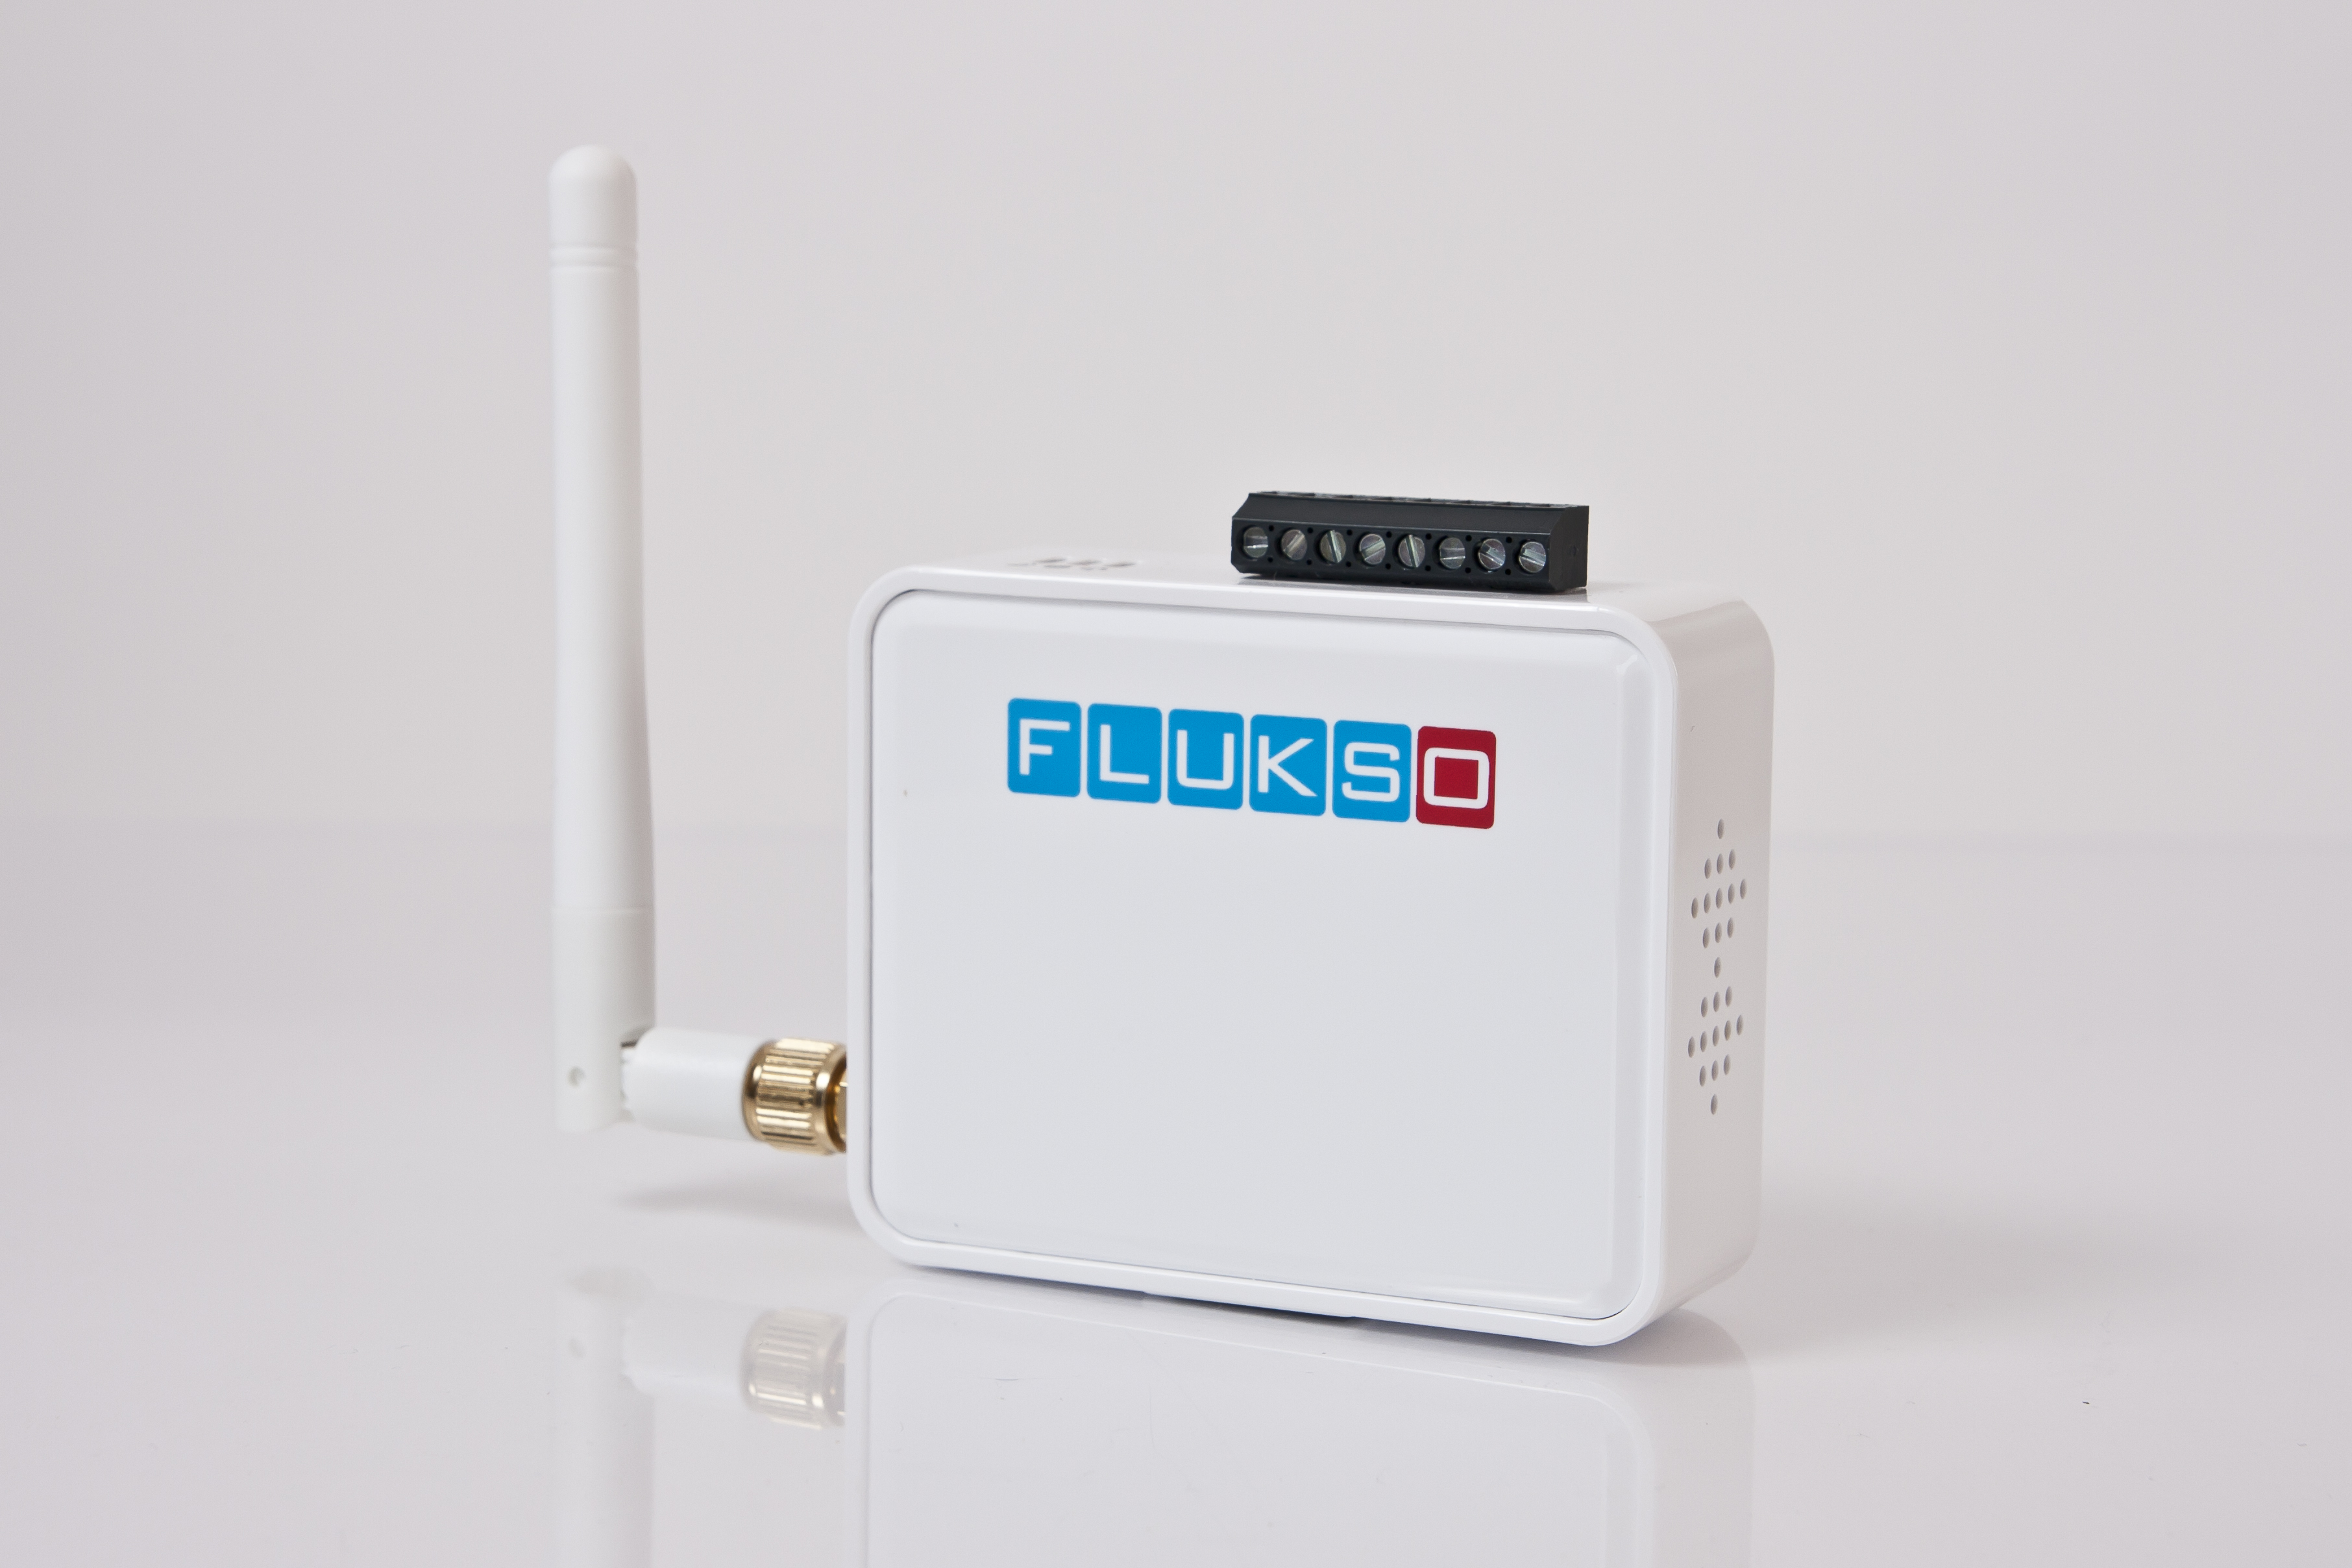
\includegraphics[width=\imgwidth]{figures/Flukso.jpg}
    \caption{Der Flukso ist ein Strommessgerät. An den Schraubklemmen
    an der Oberseite werden die Sensoren angeschlossen. Für die
    Kommunikation sind eine WLAN-Schnittstelle und eine
    Ethernet-Schnittstelle integriert. Quelle: CC-BY-SA-NC Mathias
    Dalheimer.}
    \label{fig:flukso}
  \end{center}
\end{figure}
Technisch ist der Flukso ein modifizierter WLAN-Router. Das System
besteht aus zwei Teilen: Ein kleiner Mikrocontroller kümmert sich um die
Messwerterfassung. Die Installation erfordert keine Neuverkabelung, da
die Messung indirekt über Halleffektsensoren erfolgt. Diese können
einfach um die existierenden Phasenzuleitungen gelegt werden. Die
Sensoren geben eine Spannung zwischen 0V und 5V aus, die proportional
zum Strom in den Phasenleitungen ist. Der Mikrocontroller misst diese
Spannung und rekonstruiert den aktuellen Stromverbrauch. Über die
serielle Schnittstelle werden diese Messwerte an das WLAN-Routerboard
übertragen. 

Das Routerboard basiert auf einem Atheros-Chipsatz und läuft unter
OpenWRT. Die Messdaten des Mikrocontrollers werden von einem Lua-Script
entgegengenommen, aufbereitet und dann zur mySmartGrid-Webseite
übertragen, wo sie visualisiert werden können. Ausserdem können die
Messwerte auch lokal abgefragt werden.

Die Daten werden auf der mySmartGrid-Webseite nicht dauerhaft
gespeichert, sondern nach und nach vergessen. Für die erste Stunde sind
Minutenwerte gespeichert, für die letzten 24 Stunden nur noch
fünfminütige Werte. Danach sinkt die Auflösung rapide. Wer die Daten
dennoch in hoher Auflösung haben möchte, muss die API der Webseite
benutzen. Weil viele Teilnehmer dies tun möchten, haben wir auch einen
"`Rekorder-Dienst"' implementiert, welcher die Daten in höchster
Auflösung mitschreiben kann. Die API ist als RESTful Webservice
umgesetzt und liefert die verfügbaren Daten im JSON-Format.

Die Webseite bietet auch die Möglichkeit, seine eigenen
Stromverbrauchswerte anderen Benutzern der Webseite zugänglich zu
machen. Diese können dann die eigenen Stromkurven mit denen von
anderen Benutzern vergleichen. Obwohl dies erhebliche
Privacy-Implikationen hat, geben die meisten Benutzer ihre
Stromverbrauchswerte frei. Der Vergleich des eigenen Stromverbrauchs mit
anderen Teilnehmern wird im Forum diskutiert.

Natürlich kann man nun argumentieren, dass die Daten eigentlich nicht
übertragen werden müssen. Wir gehen diesen Weg, damit auch unbedarfte
Projektteilnehmer eine schnelle Visualisierung ihrer Daten in Anspruch
nehmen können, ohne eine eigene Infrastruktur betreiben zu müssen. Mit
dem Volkszähler~\cite{web:volkszaehler} ist eine Alternative zum Flukso
verfügbar, bei der die anonyme Speicherung von Daten im Vordergrund
steht. Es ist auch denkbar, alle Messdaten lokal bei den
Teilnehmern aufzubereiten. Dies würde dann auf dem Chumby (s.u.)
geschehen. Zur langfristigen Datenspeicherung sind die in unseren
Geräten verbauten Flashspeicher allerdings nicht geeignet. Falls in
Zukunft kleine und billige SSD-basierte Speicher verfügbar sind, kann
einfach auf eine lokale Datenhaltung umgestellt werden.

Aber auch die kommerziellen und von den Messstellenbetreibern
eingesetzten Smart Meter müssen eine lokal auslesbare
Kundenschnittstelle bieten~\cite{bundesnetzagentur10position}. 
Prinzipiell ist es natürlich möglich, die Smart
Meter in die mySmartGrid-Infrastruktur anzubinden. Über die optische
serielle Kundenschnittstelle wird jede Sekunde ein Datagramm mit allen
relevanten Informationen gesendet. Ein Mikrocontroller mit zugehöriger
Fotodiode ist prinzipiell alles, was zum Auslesen benötigt wird --- eine
Open-Source Lösung hierfür fehlt derzeit.
Die momentan verfügbaren Ausleseköpfe sind entweder als
USB-Adapter oder auch als Wireless MBUS-Komponenten ausgelegt. Eine
direkte Übermittlung der Daten zur mySmartGrid-Webseite erfordert also
noch weitere Komponenten. Die Erfassung über den Flukso ist momentan die
preiswerteste Variante.

Hinzu kommt, dass die Umsetzung der Kundenschnittstelle zunächst dem
Hersteller des Stromzählers überlassen ist. Viele Hersteller setzen auf den
elektronischen Einheitszähler, der vom VDE 
standardisiert wird~\cite{fnn10lastenheft}. Aber
selbst hier finden sich Inkompatibilitäten in den Umsetzungen ---
derzeit ist kein einheitlicher Übertragungsstandard für die lokale
Schnittstelle absehbar.

Das Messen ist allerdings zumeist nicht genug, um eine nachhaltige
Änderung des Stromverbrauchsverhaltens anzuregen. Dazu setzen wir auf
zwei Ansätze:

\begin{enumerate}
  \item Automatisierte Analysen helfen, den eigenen
    Stromverbrauch zu beurteilen. Dazu sind zunächst recht fein
    aufgelöste Stromverbrauchswerte nötig, um einzelne Verbraucher
    erkennen zu können. Daher muss dieses Verfahren optional bleiben und
    nur bei Bedarf vorgenommen werden. Wir schneiden dann für zwei
    Wochen die Stromverbrauchswerte mit und identifizieren einzelne
    Verbraucher. Basierend auf dieser Analyse ist es dann recht einfach,
    konkrete Handlungsempfehlungen zu geben, z.B. "`Tauschen Sie Ihren
    Kühlschrank aus --- das amortisiert sich nach $2,4$ Jahren."' 
    Diese Analysen sind im Moment noch im Forschungsstadium.
  \item Weiterhin ist es für Stromkunden hilfreich, den Effekt ihrer
    Handlungen unmittelbar zu sehen~\cite{darby2006feedback}. Ein Wasserkocher 
    verbraucht in etwa 2kW - das führt zu einem
    gut sichtbaren Sprung in der Stromverbrauchskurve. Die logische
    Konsequenz wäre es, nur die wirklich benötigte Menge Wasser in den
    Wasserkocher zu füllen und das Wasser wirklich zu benutzen.
\end{enumerate}

Zur lokalen Anzeige der Verbrauchsinformationen bekommen die Teilnehmer
zusätzlich auch einen "`Chumby"', vgl. Abbildung \ref{fig:chumby}. 
\begin{figure}[htbp]
  \begin{center}
    
\includegraphics[width=\imgwidth]{figures/chumby.jpg}
    \caption{Der Chumby zeigt kleine Widgets an: Wetterbericht,
    Nachrichten und zukünftig auch den Stromverbrauch. Mit dem
    integrierten Internetradio ist er optimal als Küchenradio
    einzusetzen. Bild: CC-BY-SA-NC Mathias Dalheimer.}
    \label{fig:chumby}
  \end{center}
\end{figure}
Der Chumby basiert technisch ebenso wie der Flukso auf einem
WLAN-Router, hat allerdings einen Touchscreen und einen Lautsprecher
integriert. Es sind schon viele Applikationen für den Chumby verfügbar,
sodass das Gerät neben Stromverbrauchsinformationen auch den
Wetterbericht anzeigen und Internetradio abspielen kann. Da der Chumby
permanent angeschaltet ist, kann er im Hintergrund Informationen
anzeigen. Diese müssen auf einen Blick verständlich sein. Das Ziel ist
hier, eine permanente Verbrauchsanzeige zu realisieren.  Welche
Darstellungsformen für die Strominformationen am Sinnvollsten sind,
werden wir in der kommenden Zeit zusammen mit unseren Projektteilnehmern
erarbeiten. Zusätzlich wird der Chumby auch als Schaltzentrale für den
Haushalt genutzt, siehe Abschnitt \ref{sub:steuern}.

Auch für andere Anwendungen ist die Messung von Stromverbräuchen
interessant. Für die Eigentümer von Photovoltaik-Anlagen werden wir in
Zukunft spezielle Monitoring-Möglichkeiten anbieten. Dabei wird über
eine lokale Wettervorhersage der mögliche Ertrag für den kommenden Tag
prognostiziert und dann mit der tatsächlichen Produktion verglichen.
Kommt es hier zu größeren Abweichungen, kann der Eigentümer der Anlage
verständigt werden. Diese Informationen lassen sich auch zur Optimierung
des Eigenstromverbrauchs verwenden: Wenn sich abschätzen lässt, wann
entsprechende Strommengen produziert werden, kann man Hinweise zur
Steuerung von Stromverbrauchern geben. So lässt man dann die
Waschmaschine vielleicht nicht morgens, sondern mittags laufen, wenn
einen Tag im Voraus klar ist, wann die Sonne scheinen wird.

\subsection{Regelung von Verbrauchern}\label{sub:steuern}

Der nächste Schritt ist das automatische Steuern von Verbrauchern im
Haushalt. Mit Hilfe von meteorologischen Modellen ist es möglich, die
Stromproduktion auf Tagesfrist recht genau vorherzusagen. Wenn also
morgen Mittag der Wind weht oder die Sonne scheint, führt dies auch zu
einer erhöhten Stromproduktion. Diese Information kann dann einen Tag im
Voraus zu den Haushalten transportiert und angezeigt werden. Die Nutzer
können ihr Verhalten entsprechend anpassen --- für eine Spülmaschine ist
es meist recht egal, ob sie morgens oder mittags läuft.

Natürlich ist dies aber nicht genug, denn eigentlich sollte diese
Regelung automatisch passieren. Leider bieten die meisten
Haushaltsgeräte keine Möglichkeit, Steuerbefehle à la "`heute mittag um
14:00 Strom verbrauchen"' zu verarbeiten. Ebenso ungelöst ist die Frage
nach einem universellen und nachrüstbaren Bussystem, welches diese
Steuerinformationen zu den Verbrauchern transportiert. Bussysteme wie
EIB und KNX sind nur dann sinnvoll einsetzbar, wenn gleichzeitig größere
Umbauten an der Wohnung vorgenommen werden. Darüber hinaus sind diese
Systeme auch recht teuer. Dies schließt alle Leute aus, die in einer
Mietwohnung wohnen, denn beim Auszug ist es nicht ohne weiteres
möglich, das Bussystem mitzunehmen.

Mit "`digitalStrom"' wird derzeit ein anderes System entwickelt, welches
mit relativ geringem Aufwand nachrüstbar ist und Steuerinformationen
über das Stromnetz transportiert. Dieses System ist jedoch noch nicht am
Markt verfügbar --- die Markteinführung wurde in den vergangenen Jahren
immer wieder verschoben. Ausserdem ist das digitalStrom-System eine
proprietäre Lösung, die nur von einem Anbieter angeboten wird. 

Langfristig ist eine Lösung wünschenswert, die eine IP-basierte
Kommunikationsinfrastruktur auf kleinen Mikrocontrollern umsetzt. Eine
solche Lösung wäre bezahlbar, gleichzeitig könnte durch die Verwendung
von IPv6 das Problem der Adressvergabe an die Endgeräte gelöst werden.
Unsere Prototypen auf der Basis von 6LoWPAN und funkbasierter Kommunikation
(868 MHz) zeigen, dass eine solche Lösung sehr wohl
kostengünstig umzusetzen ist\footnote{Eine komplette Dokumentation
inklusive Kalkulation der Materialkosten des
Prototyps ist unter
\url{http://developer.mysmartgrid.de/doku.php?id=project_octobus}
beschrieben.}.
\begin{figure}[htbp]
  \begin{center}
    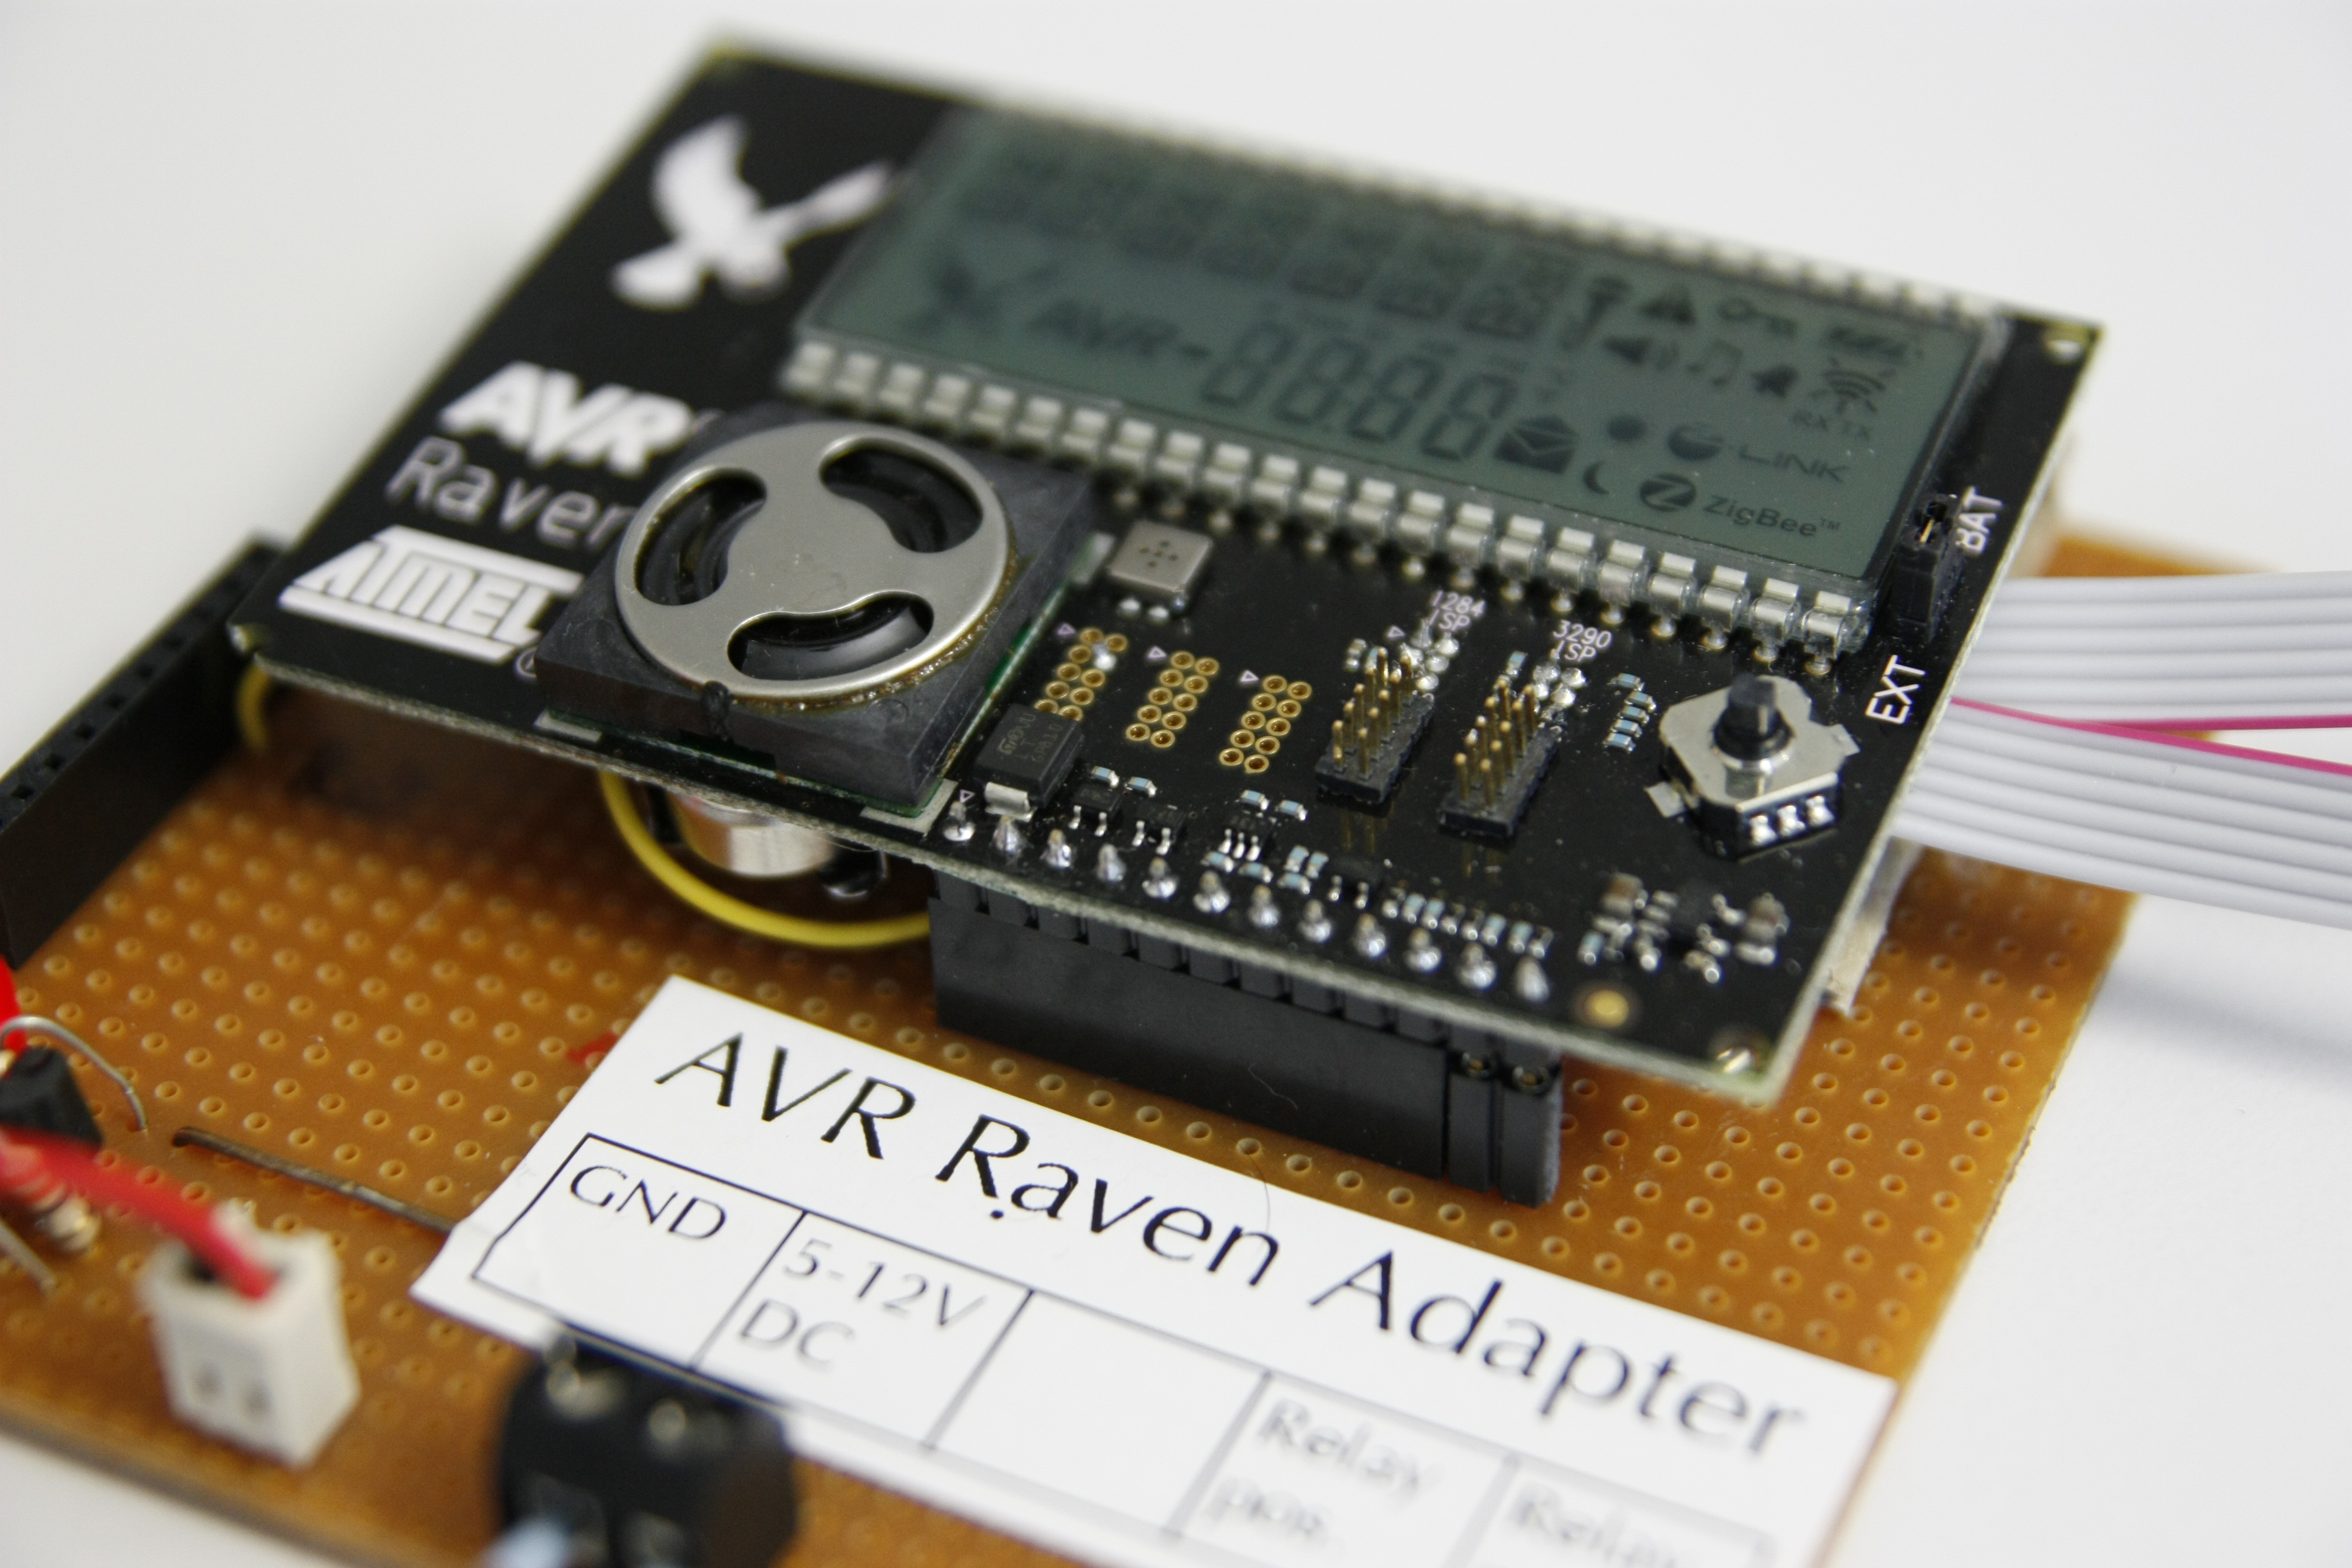
\includegraphics[width=\imgwidth]{figures/raven-adapter.JPG}
    \caption{Logikteil des OctoBus-Prototyps, basierend auf dem AVR
    Raven Evaluation Kit. Auf dem Kit läuft Contiki. Ein externes Relais
    wird geschaltet, wenn ein entsprechendes UDP-Paket empfangen wird.
    Bild: CC-BY-NC-SA Mathias Dalheimer}
    \label{fig:raven-adapter}
  \end{center}
\end{figure}
Der Prototyp "`OctoBus"' kann derzeit von beliebigen IPv6-Rechnern aus
ein Relais schalten, siehe Abb. \ref{fig:raven-adapter}.  Als
Betriebssystem benutzt OctoBus Contiki~\cite{yazar09efficient}.
Alternativ ist auch mit Ethersex eine etablierte Lösung
verfügbar~\cite{web:ethersex}. Da hochintegrierte Funkchipsätze sowie leistungsfähige
8Bit-Mikrocontroller verfügbar sind, kann eine
Funkschaltsteckdose für 20 Euro Materialkosten hergestellt werden.
Momentan arbeiten wir mit Partnern daran, eine Kleinserie von 300
Funkschaltsteckdosen-Sets zu entwickeln und zu fertigen. Diese Technik
wird dann auch in unseren Teilnehmerhaushalten installiert.

Für das Projekt optimal sind Haushaltsgeräte, die einerseits recht viel
Strom im Betrieb verbrauchen und bei denen andererseits das Verzögern
des Betriebs möglich ist. Realistische Geräte für diese Anwendung sind
also Waschmaschinen und Spülmaschinen, aber auch Tiefkühlgeräte oder
Wärmepumpen. Sowohl Waschmaschinen als auch Spülmaschinen sind
allerdings nicht einfach einzubinden, da diese vor dem Betrieb natürlich
beladen werden müssen und eventuell auch ein Wasserhahn geöffnet werden
muss. Daher liegt der Schwerpunkt unserer Arbeit zunächst einmal auf
Kühlgeräten und Wärmepumpen. Die Einbindung von weiteren Geräten
(vlg. \cite[S. 22]{wiechmann08lastmanagement}) ist aber vorgesehen.

Wir greifen dabei nicht in die interne Regelung der Geräte
ein\footnote{Es wäre für unsere Teilnehmer wohl nicht akzeptabel,
Haushaltsgeräte konstruktiv zu verändern.}. Für
Kühlschränke und Gefriertruhen funktioniert folgenden Ansatz: Die
Geräte werden über einen Zwischenstecker von der Stromversorgung
getrennt. In der Folge steigt die Innentemperatur an. Wenn nun der
Stromverbrauch zu einem Zeitpunkt $t$ maximiert werden soll, muss die
Innentemperatur zu diesem Zeitpunkt also recht hoch sein. Dann wird das
Kühlgerät wieder ans Netz angeschlossen. Die Regelung des Kühlgerätes
wird nun aufgrund der (relativ) hohen Innentemperatur den Kompressor
anschalten und wie gewünscht Strom verbrauchen. Diese Herangehensweise
darf jedoch nicht dazu führen, dass Lebensmittel verderben oder
Tiefkühlware auftaut.

Eine einfache Lösung wäre, die Innenraumtemperatur des Kühlgerätes über
einen Sensor zu überwachen. Dieser Sensor verursacht jedoch
Zusatzkosten. Daher prognostizieren wir das Verhalten der internen
Regelung des Gerätes und übersteuern diese gezielt. Das setzt eine
Systemidentifikation und eine Einrichtungsprozedur voraus. Diese
ermittelt dann Regelparameter, die dazu benutzt werden, das Kühlgerät
gezielt vor dem geplanten Anschaltzeitpunkt auszuschalten. Gleichzeitig
ist gewährleistet, dass die Kühlkette nicht unterbrochen wird. Aus den
Strommessungen lässt sich lokal auch feststellen, ob der Kompressor
eines Kühlgerätes anläuft. Durch kurzes Einschalten ist es auch ohne
Temperatursensor möglich, Rückschlüsse auf die Innentemperatur des
Kühlgerätes zu ziehen. Die Technik hierfür funktioniert schon. Da aber
im Moment noch kein brauchbares Hausbussystem zur Verfügung steht, sind
derzeit nur zwei Testkühlschränke entsprechend ausgerüstet. Für
Wärmepumpen funktioniert der gleiche Ansatz, die entsprechende
Regelungstechnik wird derzeit entwickelt.

Der wichtigste Faktor ist jedoch die Akzeptanz der Technologie bei den
Anwendern: Diese müssen jederzeit in der Lage sein, die vorgeschlagenen
Regeleingriffe abzulehnen. Da die Regelungsalgorithmen sowieso auf dem
Chumby laufen werden, ist hier auch der logische Platz, um den Benutzer
über die aktuelle Planung zu informieren. Dort wird es dann auch die
Möglichkeit geben, die Regelung zu beeinflussen oder auch zu
deaktivieren. Sobald entsprechende Schnittstellen zu weiteren Geräten
verfügbar sind, spricht natürlich auch nichts dagegen, diese
einzubinden.

Schliesslich ist eine weitere Gruppe von Stromkunden sehr interessant
für den Einsatz von Haussteuerungen: Für Photovoltaikanlagenbesitzer ist
ab diesem Sommer der Eigenverbrauch des selbst erzeugten Stroms die
rentabelste Option, wenn die Anlage nach dem 1. Juli 2010 ans Netz geht.
Dafür ist es notwendig, Haushaltsgeräte möglichst dann zu betreiben,
wenn die Photovoltaikanlage auf dem Dach gerade Strom liefert. Für jede
selbst erzeugte und selbst verbrauchte Kilowattstunde (am 30~\%
Eigenverbrauchsanteil) bekommt der Anlagenbesitzer $0,22~{\euro}/{kWh}$.  Dazu
kommen natürlich noch circa $0,20~{\euro}/{kWh}$, die gespart werden, weil der
Strom nicht über den Hausanschluss von aussen eingekauft werden muss. Im
Vergleich dazu bekommt der Anlagenbesitzer maximal $0,34~{\euro}/{kWh}$, wenn
eine Kilowattstunde selbst erzeugten Stroms in das Netz eingespeisst
wird.  Unter dem Strich kann der Anlagenbesitzer also $0,08
~{\euro}/{kWh}$ mehr
einnehmen, wenn der Strom selbst verbraucht wird. In Zukunft werden die
Zuschüsse weiter sinken, die Relationen zwischen Einspeisung und
Eigenverbrauch werden jedoch gleich bleiben. Dies macht auch ökonomisch
Sinn, denn der selbstverbrauchte Strom muss nicht über das Stromnetz
transportiert werden und entlastet es. Ein teurer Netzausbau kann so
vielleicht nicht ganz vermieden, aber doch verzögert bzw.  reduziert
werden.

Praxistauglich ist so ein System nur, wenn vorab bekannt ist, wann die
Photovoltaikanlage Strom liefert und wann nicht. Daher müssen
Wetterprognosen in die Regelung der Geräte einbezogen werden, um den
optimalen Betriebszeitpunkt zu ermitteln. Diese können dann auch auf dem
Chumby angezeigt werden, sodass die Haushaltsbewohner diese
Informationen bewusst in ihr Nutzungsverhalten einbeziehen können.

Die Hersteller von Wechselrichtern für Solaranlagen sind dabei,
entsprechende Managementfunktionen in ihre Geräte zu integriern. Dabei
rechnen sie damit, dass zwischen 30 und 50~\% des eigenen Solarstroms
selbst verbraucht werden können~\cite{ossenbrinck10herstellung}. Die
Geräte hierfür werden zwischen 700 und 900 Euro kosten und zusätzlich
zum Wechselrichter installiert werden. Auch hier werden Tiefkühlgeräte
als regelbare Geräte eingebunden~\cite{ossenbrinck10herstellung}.

%TODO: Lösung von Conergy kostet 850-900 Euro. Rentabilität? Nur für
%diesen einen Zweck einsetzbar?
%
%Ausserdem: Connergy will 2011 auch Energiespeicher für Zuhause anbieten
%(Li-Ion, 8kWh). Lebensdauer > 20 Jahre.
%
%IBC Solar: 700 Euro, Amortisation nach 5-7 Jahre bei einer 5kWp-Anlage.
%
%Als Geräte favorisieren sie Tiefkühlanlagen.
%

Basierend auf den hier dargestellten Projektergebnissen gehen wir davon
aus, eine entsprechende Überwachungsfunktionalität --- je nach Ausbaustufe ---
zwischen 150 und 400 Euro anbieten zu können. Dazu kommt dann noch ein
Datenabo, da die Wetterprognosen in die Geräteüberwachung einfließen.
Dabei ist unsere Lösung herstellerunabhängig.

\subsection{Virtueller Verbraucher}\label{sub:virtuellerverbraucher}
Natürlich ist es für einen einzelnen Haushalt nicht möglich,
signifikanten Einfluss auf das Stromnetz zu haben. Allerdings gibt es ja
recht viele Haushalte, auf die man potentiell Einfluss nehmen könnte.
Alle Teilnehmer rufen also einen Tag im Voraus die Prognose für den
nächsten Tag ab und versuchen, diese umzusetzen. Zusammen genommen sind
1000 Haushalte dann in der Lage, vielleicht 1~MWh zu verschieben.  Die
genaue Modellierung ist hier ein statistisches Problem, denn nicht jeder
Haushalt wird sich an die Handlungsempfehlungen halten. Zusammengenommen
dürfte es jedoch möglich sein, einen signifikanten Einfluss auf das
lokale Stromnetz zu haben.

Dieser Eingriff bietet Chancen für die lokalen Netzbetreiber. Diese
können dieses Regelpotential in ihre kurzfristige Planung mit
einbeziehen. Wenn normalerweise Lastspitzen durch den teuren,
kurzfristigen Zukauf von Strom abgedeckt werden müssen, können sie durch
die Verschiebung von Lasten Geld sparen. Diesen Profit können sie sich
dann mit den teilnehmenden Haushalten teilen. Hier sind zwei Modelle denkbar: 
\begin{enumerate}
  \item Die Haushalte schliessen sich zu einer Genossenschaft zusammen
    und verhandeln direkt mit dem lokalen Netzbetreiber. Die Vermarktung
    des Regelpotentials ist nicht an einen Stromlieferanten gebunden,
    d.h. die Eigner der Genossenschaft können ihren Strom bei
    unterschiedlichen Lieferanten einkaufen. Die Einnahmen der
    Genossenschaft können zur Finanzierung der Geräte verwendet werden.
    Dieses Modell macht dort Sinn, wo kleinere Netzbetreiber wie
    unabhängige Stadtwerke den Netzbetrieb organisieren.
  \item Ein anderes Modell wäre die Finanzierung der Geräte etc. über
    den Stromvertrieb, d.h. ein Stromkunde bekommt andere
    Lieferkonditionen, wenn er mit der Regelung seiner Geräte
    einverstanden ist. Hier hat der Stromkunde gegenüber dem
    Genossenschaftsmodell eine schwächere Position. Zudem ist dieses
    Modell aufgrund der Organisation des Strommarkts schwierig
    umzusetzen.
\end{enumerate}

Für mySmartGrid favorisieren wir das Genossenschaftsmodell. Nach
Projektende werden wir die Geräte aus dem Projekt bei den Teilnehmern
belassen und die Gründung einer Genossenschaft fördern. Derzeit sind wir
jedoch noch nicht soweit, dass wir ein abschliessendes Konzept für ein
Geschäftsmodell haben.

Ein alternatives Konzept --- das derzeit auch meistens im Rahmen der
E-Energy-Projekte diskutiert wird --- sind flexible Stromtarife. Dabei
ändert sich der Preis für eine Kilowattstunde Strom in Abhängigkeit
davon, wie die Situation im Stromnetz gerade ist. Die Stromkunden sollen
dann ihre Geräte entsprechend steuern. Im Gegensatz zu einem virtuellen
Verbraucher stärkt das Konzept flexibler Strompreise jedoch die großen
Stromanbieter und damit die gegenwärtigen Marktstrukturen. Ein virtueller
Verbraucher verlagert hingegen die Marktmacht in Richtung der
Stromkunden und kleineren Stadtwerke.

Nicht vergessen darf man an dieser Stelle auch die Probleme des Systemdesigns:
Als großes verteiltes System muss die Umsetzung zu einem stabilen
Systemverhalten führen. Ausfälle von einzelnen Systemkomponenten dürfen
nicht zu Störungen des Gesamtsystems führen.  Wir favorisieren 
einen dezentralen Ansatz: Steuergeräte in den einzelnen Haushalten
verhalten sich dabei autonom und lassen sich jederzeit von den Bewohnern
beeinflussen. Lediglich ein gewünschtes Lastprofil wird
den Haushalten vorgegeben. Die einzelnen Haushalte entscheiden dann
autonom, wie einzelne Geräte zu steuern sind.  Die Verteilung des
Lastprofils kann dabei durch standardisierte Protokolle über das
Internet erfolgen.


\section{Schlussfolgerungen}
Das Smart Grid, "`intelligentes Stromnetz"', ist eines der Themen, welche
von der Politik und natürlich auch der Stromwirtschaft immer wieder in
den Vordergrund gestellt werden. Das Potential der erneuerbaren Energien
reicht aus, um Deutschland und Europa zuverlässig mit Strom zu
versorgen~\cite{sachverst10erneuerbar}. Der Umbau der Stromnetze ist
dabei von zentraler Bedeutung und bedarf einer Anstrengung der gesamten
Gesellschaft. Leider kommt dabei der Stromkunde zu
kurz --- die Bedürfnisse von Stromkunden werden weitgehend ignoriert und
der Datenschutz wird oft ausser acht gelassen~\cite{web:bmwinutzerschutz}.

Aber auch kleinere Stadtwerke haben mit dieser Entwicklung Probleme:
Aufgrund politischer Vorgaben müssen sie zum Beispiel Smart Meter
einführen, obwohl ihnen dadurch Kosten entstehen, die sie nicht direkt
auf den Kunden umlegen können. Die Bereitschaft der Kunden, für ein
Smart Grid mehr Geld zu bezahlen, ist wohl kaum vorhanden. Gleichzeitig
ist es aber notwendig, die bestehenden Stromnetze zu flexibilisieren und
auf einen weiter steigenden Anteil von erneuerbaren Energiequellen
vorzubereiten. Damit dieser Wandel funktionieren kann, müssen viele
Rahmenbedingungen beachtet werden:

\begin{enumerate}
  \item \emph{Kunden} müssen im Endeffekt diesen Wandel bezahlen. Daher
    sollten alle Änderungen auch im Sinne des Kunden gestaltet werden.
    Die im Moment verfügbaren Lösungen sind oft zu teuer und werden eher
    als Lifestyle-Produkt vermarktet. Hier gibt es noch erhebliches
    Potential.
  \item Die Rolle der \emph{Stadtwerke} und kleinen Verteilnetzbetreiber
    wird wichtiger werden. Hier besteht wiederum die Chance, dass diese
    -- oft in kommunaler Hand befindlichen -- Unternehmen
    partnerschaftlich mit Kunden und kleineren Energieerzeugern kreative
    Lösungen erarbeiten.
  \item Schliesslich müssen auch rechtliche Rahmenbedingungen im
    Interesse der Kunden gestaltet werden. Die derzeitige Debatte um die
    Laufzeitverlängerungen für Atomkraftwerke zeigt, dass politische
    Entscheidungen nicht immer zu langfristig guten Lösungen führen und
    auch die meisten Expertenaussagen nicht beachtet wurden. Hier müssen
    konstruktive Vorschläge erarbeitet und auch an die politischen
    Entscheidungsträger kommuniziert werden.
\end{enumerate}

Das Stromnetz ist ein historisch gewachsenes System. Viele
unterschiedliche Konzepte wurden kombiniert, ebenso wurden viele
rechtliche Rahmenbedingungen geschaffen. Insofern ist eine Veränderung
nur in kleinen Schritte möglich. Einzelne Komponenten werden
nacheinander ausgetauscht und müssen natürlich gleichzeitig ein Teil des
Gesamtkonzepts werden.

Für dieses Problemfeld bieten sich Open Source-Lösungen an: Diese können
aufgrund der offenen Spezifikationen und Quellcodes recht schnell an
neue Gegebenheiten angepasst werden. Ebenso ist es möglich, diese
Anpassungen dezentral durch viele Anbieter vornehmen zu lassen. Diese
Flexibilität kommt sowohl den Verteilnetzbetreibern als auch den
Geräteherstellern zugute. Gleichzeitig ist es elementar, auf bereits
existierende Kommunikationsstandards wie TCP/IP zu setzen.

In diesem Bericht wurde die Thematik des Stromhandels weitgehend
ausser Acht gelassen. Hier sei auf den Bericht von Andreas Wagner
(Fraunhofer ITWM) hingewiesen~\cite{wagner11market}.

\section*{Danksagung}\label{danksagung}
Mein Dank für Anregungen und Diskussionen gilt Dr. Franz-Josef Pfreundt,
Ely Wagner Aguiar de Oliveira, Matthias Klein, Stephan Platz, Simon
Birnbach sowie Dominik Keller. Das Projekt mySmartGrid wird durch das
Land Rheinland-Pfalz im Rahmen des Konjunkturprogramm II geförtert.

\bibliographystyle{plain}
\bibliography{main}
\end{document}

